
\begin{figure}[htb]
\centering
\includegraphics[page=6,width=0.4\textwidth]{\FCNCFigures/tthML/raw/faketau/postfit/NOMINAL/reg1l1tau1b3j_os/x1fit.pdf}
\put(-140, 92){\footnotesize{TTH $\tlhad$}}
\includegraphics[page=6,width=0.4\textwidth]{\FCNCFigures/tthML/raw/faketau/postfit/NOMINAL/reg1l1tau1b3j_os/x2fit.pdf}
\put(-140, 92){\footnotesize{TTH $\tlhad$}}\\
\includegraphics[page=4,width=0.4\textwidth]{\FCNCFigures/xTFW/SSOS/NOMINAL/reg2mtau1b3jos/x1fit.pdf}
\put(-140, 92){\footnotesize{TTH $\thadhad$}}
\includegraphics[page=4,width=0.4\textwidth]{\FCNCFigures/xTFW/SSOS/NOMINAL/reg2mtau1b3jos/x2fit.pdf}
\put(-140, 92){\footnotesize{TTH $\thadhad$}}
\caption{ The distributions of $x_{1,2}^{\text{fit}}$ in the TTH $\tlhad$ (top) and $\thadhad$ (bottom) channels. }
\label{fig:x12_fit}
\end{figure}